\begin{frame}
\frametitle{Problem addressed}
\itemize
\item \tiny{\textcolor{blue}{Multiple control loops work
concurrently and share various resources including the communication
bus \footnote{\tiny{\textcolor{blue}{Through Communication bus control loops interact with sensors and actuators}}}.}} 

\item \tiny{\textcolor{blue}{A possible insider attack could be the replacement of a previously
vetted control application. }}

\item \tiny{\textcolor{blue}{ Replacements can lead to disaster.\footnote{\tiny{\textcolor{blue}{ For example, slowing down a
particular process in the industrial manufacturing can cascade 
a chain of failures in the whole
assembly line.}}}}}
\begin{figure}
\begin{center}
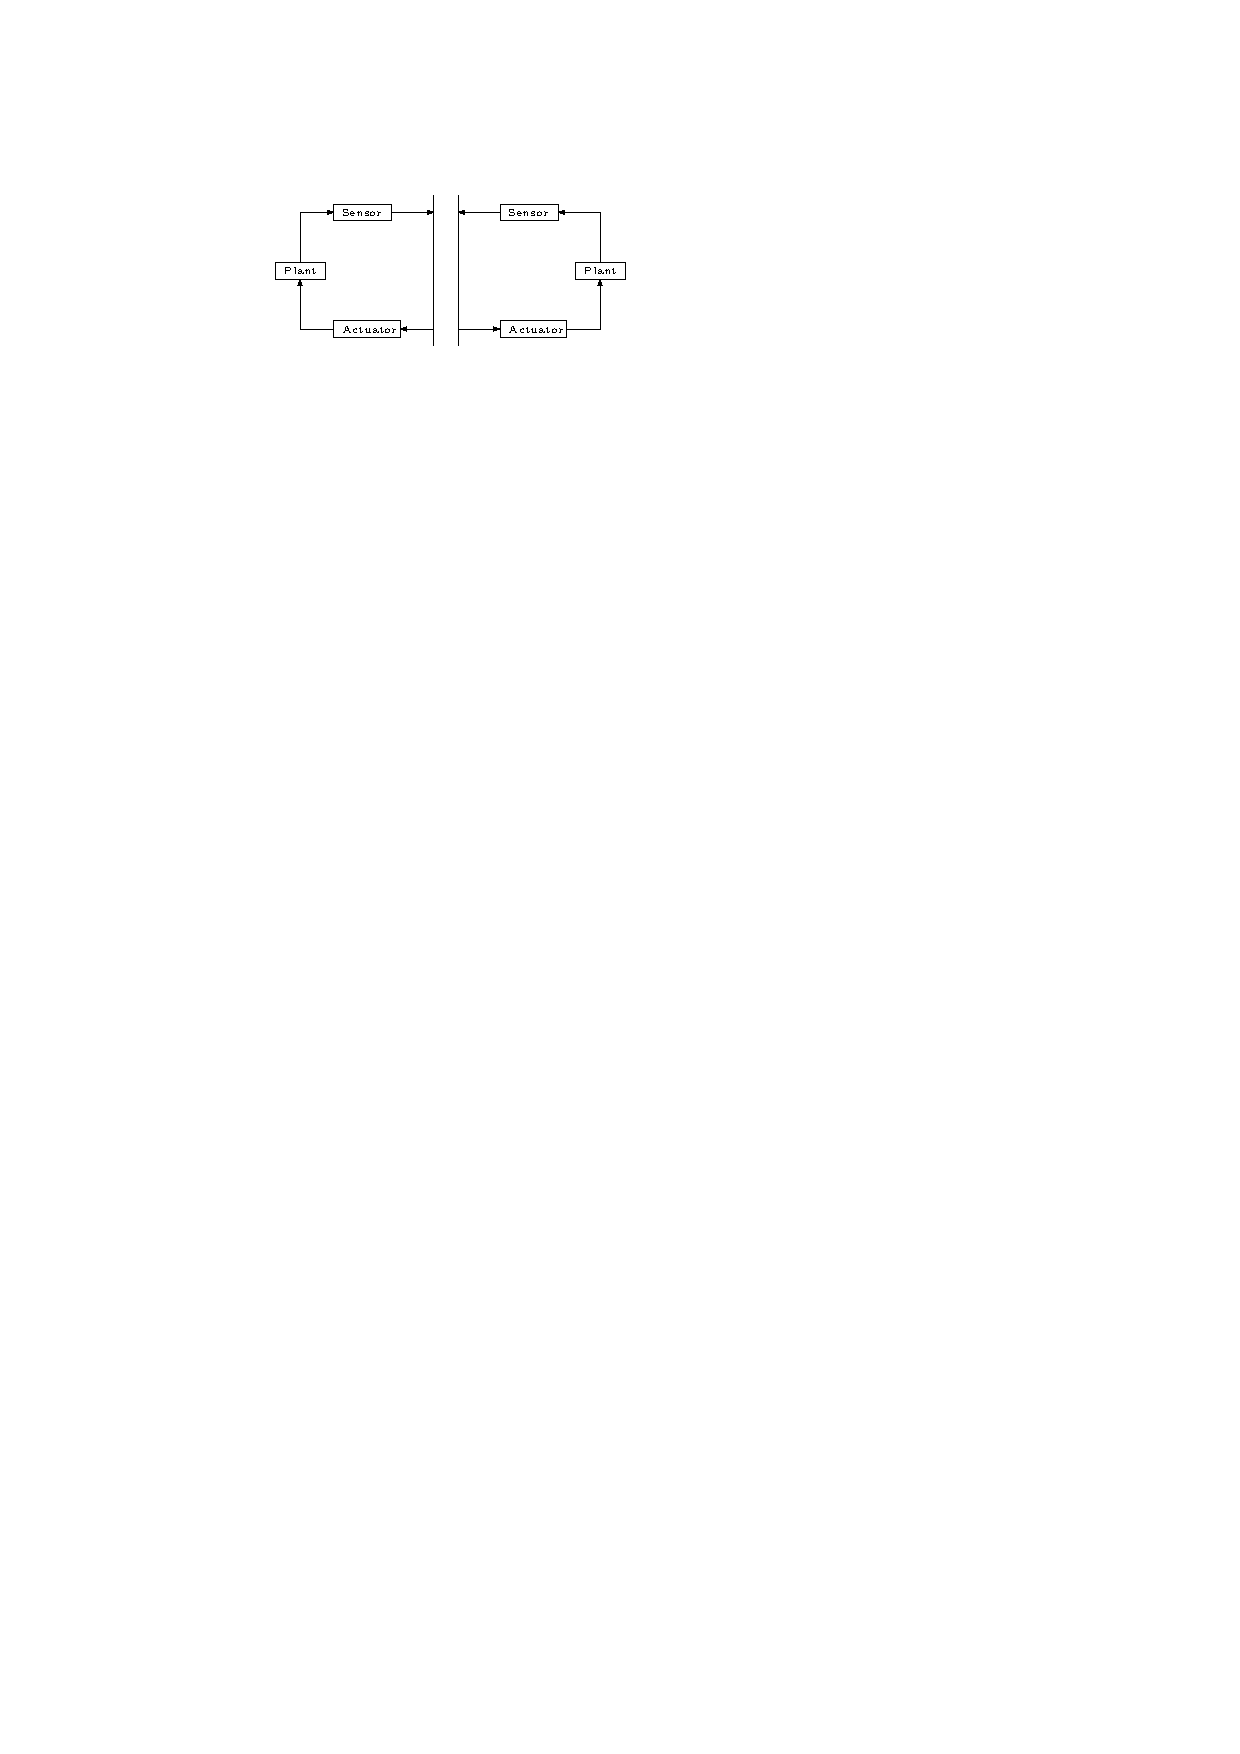
\includegraphics[width=35mm]{control_diagram.pdf}
\end{center}
%\vspace{-0.1in}
\caption{{\em \tiny{\textcolor{blue}{Control Loops}}}} \label{fig1}
\end{figure}

\item \tiny{\textcolor{blue}{Focus of this project: replacement attacks.
\footnote{\tiny{\textcolor{blue} {One or more 
control component is replaced with a modified one.}}}}}

%\item \tiny{\textcolor{blue}{ Address the problem of detecting component replacement attacks
%from the schedulability perspective.}}

%\item \tiny{\textcolor{blue}{Given a set of control components, a control objective 
%to be satisfied by the control ensemble, the question of schedulability and 
%synthesis of a scheduler that can ensure the desired control performance.}}


\item \tiny{\textcolor{blue}{Our proposal: such
attacks can be guarded against by statically analyzing the
legitimate control programs, and constructing an omega-regular language based timing signature.}}
%\footnote{\tiny\textcolor{blue}{ can then be periodically checked on the running components to distinguish a replaced
%component from the original one.}}
%The idea presented here is based on the timing signature 
%analysis for omega-regular languages~\cite{WeissFAA09}, in the context of real-time 
%communication scheduling in SCADA systems.}}



\end{frame}

%\tiny{\textcolor{blue}{In this project, we propose an automated framework
%that addresses the effect of such replacement attacks from the perspective
%of loss of control performance. Given a set of control components,
%a control objective to be satisfied by the control ensemble, the question
%of schedulability and synthesis of a scheduler that can ensure the de-
%sired control performance has been recently studied in literature. In this
%paper, we extend this idea further to build an automata theoretic frame-
%work for assessment of replacement attacks on schedulability.}}

